\label{sec:rawDataMCComparisons}

In this Section, the detector-level distributions of the jet mass
are investigated. Each of the distributions are made for 
the $\pt^{AVG}$ bins described in Section~\ref{sec:ptBinAssignment}. 
Each of the figures shows the raw event counts per $\pt^{AVG}$ bin,
as a function of the average jet mass $m_J^{AVG}$. 


Figure~\ref{figs:histAK7PtAvgVsMjetGroomOverReco_ratioPlots}
shows a comparison of the jet mass from the groomed jets
divided by the jet mass of matched ungroomed jets, for the
three grooming techniques, for both data and the \PYTHIA Monte Carlo. 
The data and the MC both exhibit similar behavior. In general,
the filtering algorithm (black) is the least aggressive grooming technique,
with groomed jet masses close to the ungroomed case.
The trimming algorithm (red) is moderately aggressive, and the
pruning algorithm (blue) is the most aggressive. In the case of
the pruning algorithm, a bimodal distribution begins to manifest,
which is typical of this algorithm since the parameters we have
chosen require two subjets to be created. In the cases where
the pruned jet mass is close to the ungroomed jet mass, 
jets usually have large ``core'' components
and small amounts of radiation, whereas when the pruned jet
mass is closer to 0, the jets are more symmetrically split
due to gluons splitting into two jets that fall within
our $D=0.7$ parameter. 


Figures~\ref{figs:controlPlots_histAK7PtAvgVsNvtx} and \ref{figs:controlPlots_histAK7DeltaPhi}
show the $\pt^{AVG}$ and $\Delta \phi$ distributions for the data
compared to the \PYTHIA MC. The $\pt^{AVG}$ distribution is reasonably
well-modeled with the \PYTHIA MC, but the $\Delta \phi$ distribution
does show some mismodeling.

Figures~\ref{figs:histAK7MjetVsPtAvg_rawDataMCComparisons_stacktrigs_pt_1}-
\ref{figs:histAK7MjetVsPtAvg_rawDataMCComparisons_stacktrigs_pt_10}
show the jet mass distribution for AK7 jets, along with
the trigger breakdown for all of the $\pt^{AVG}$ bins. In each case,
only one trigger contributes to any given $\pt^{AVG}$ bin. 

Figures~\ref{figs:histAK7MjetVsPtAvg_rawDataMCComparisons_pt_1}-
\ref{figs:histAK7MjetVsPtAvg_rawDataMCComparisons_pt_10_Pruned}
show the detector-level distributions for the various jet grooming
algorithms, compared to predictions from \PYTHIA, \PYTHIA8, and
\HERWIG Monte Carlo samples. Each MC sample is normalized
according to the expected luminosity and computed cross sections. 



\begin{figure}[htbp]
\centering
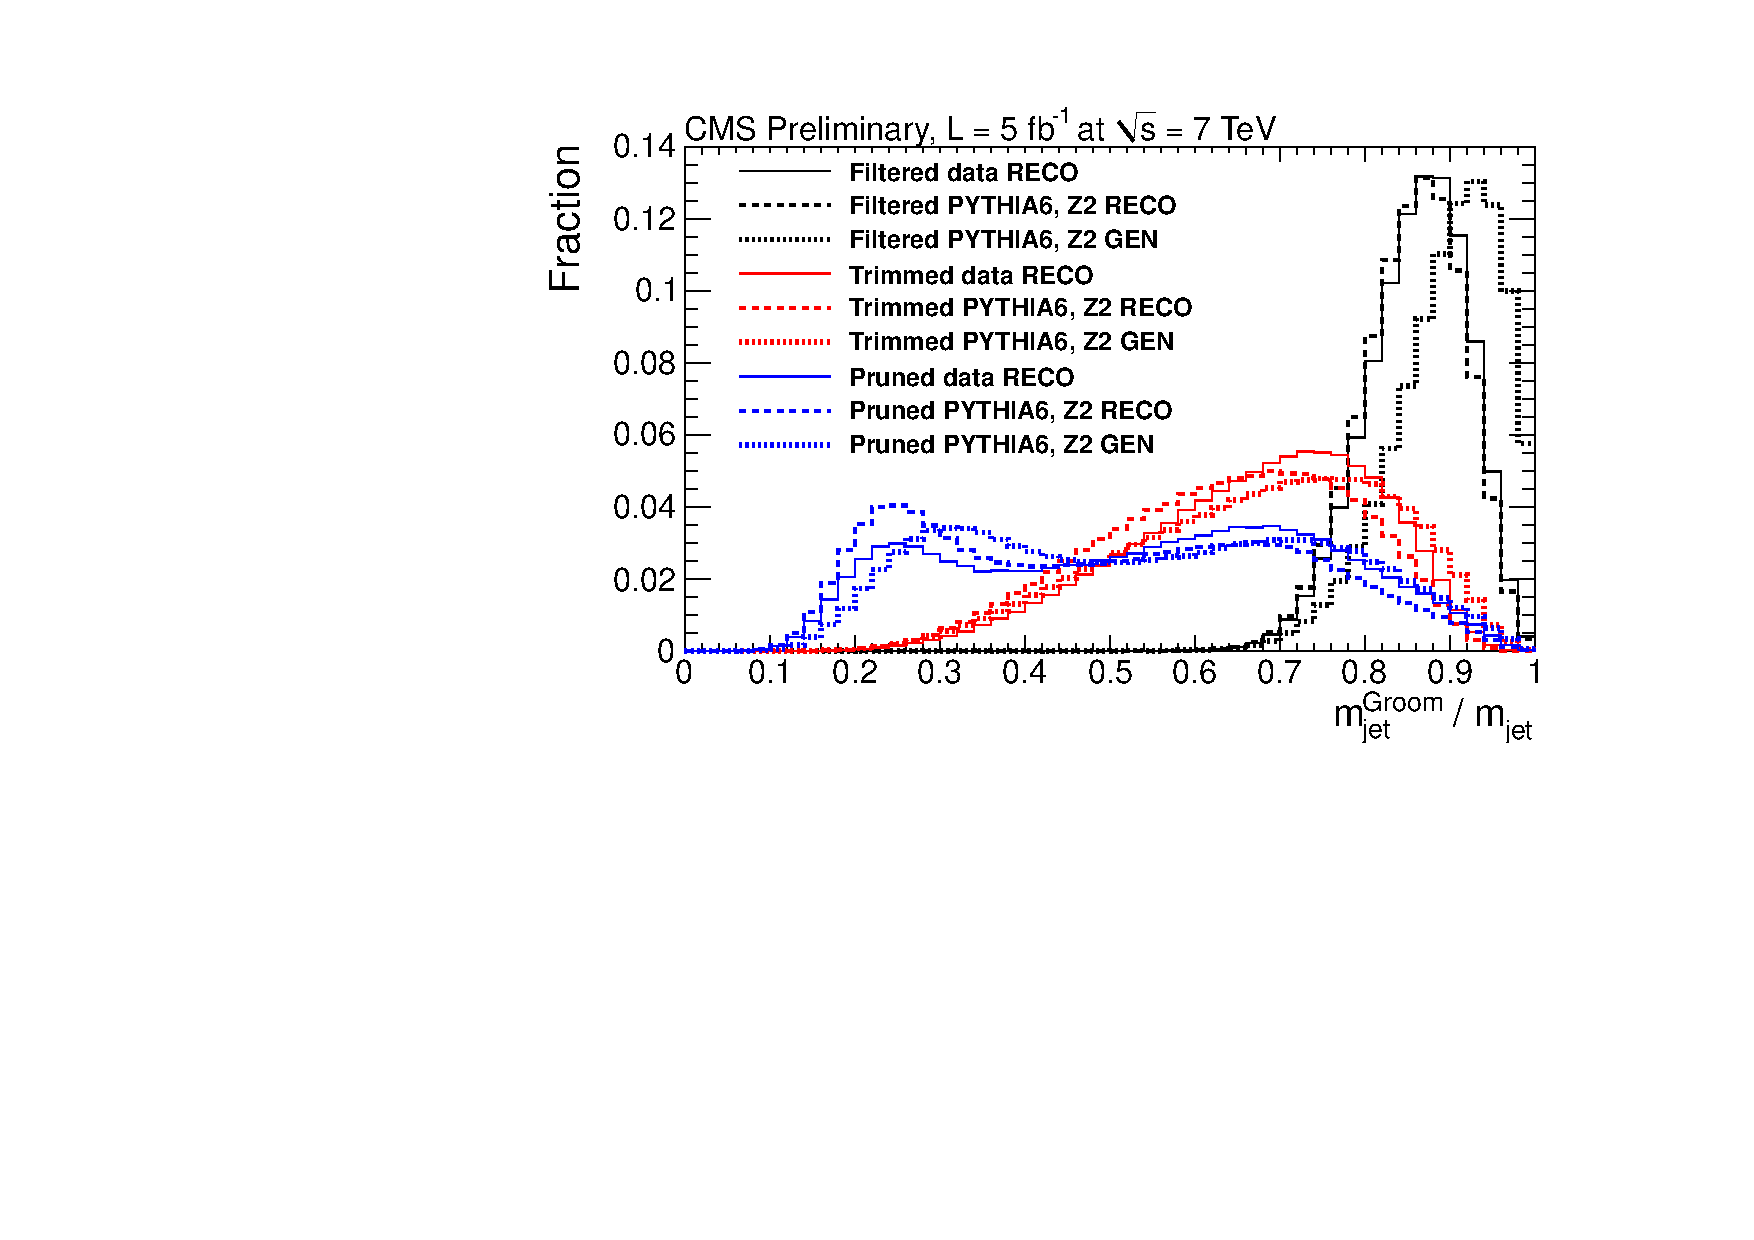
\includegraphics[width=0.95\textwidth]{figs/histAK7PtAvgVsMjetGroomOverReco_ratioPlots}
\caption{Comparison of the jet mass from the groomed jets
divided by the jet mass of matched ungroomed jets for the
three grooming techniques, for both data and the \PYTHIA Monte Carlo. 
\label{figs:histAK7PtAvgVsMjetGroomOverReco_ratioPlots}}
\end{figure}


\begin{figure}[htbp]
\centering
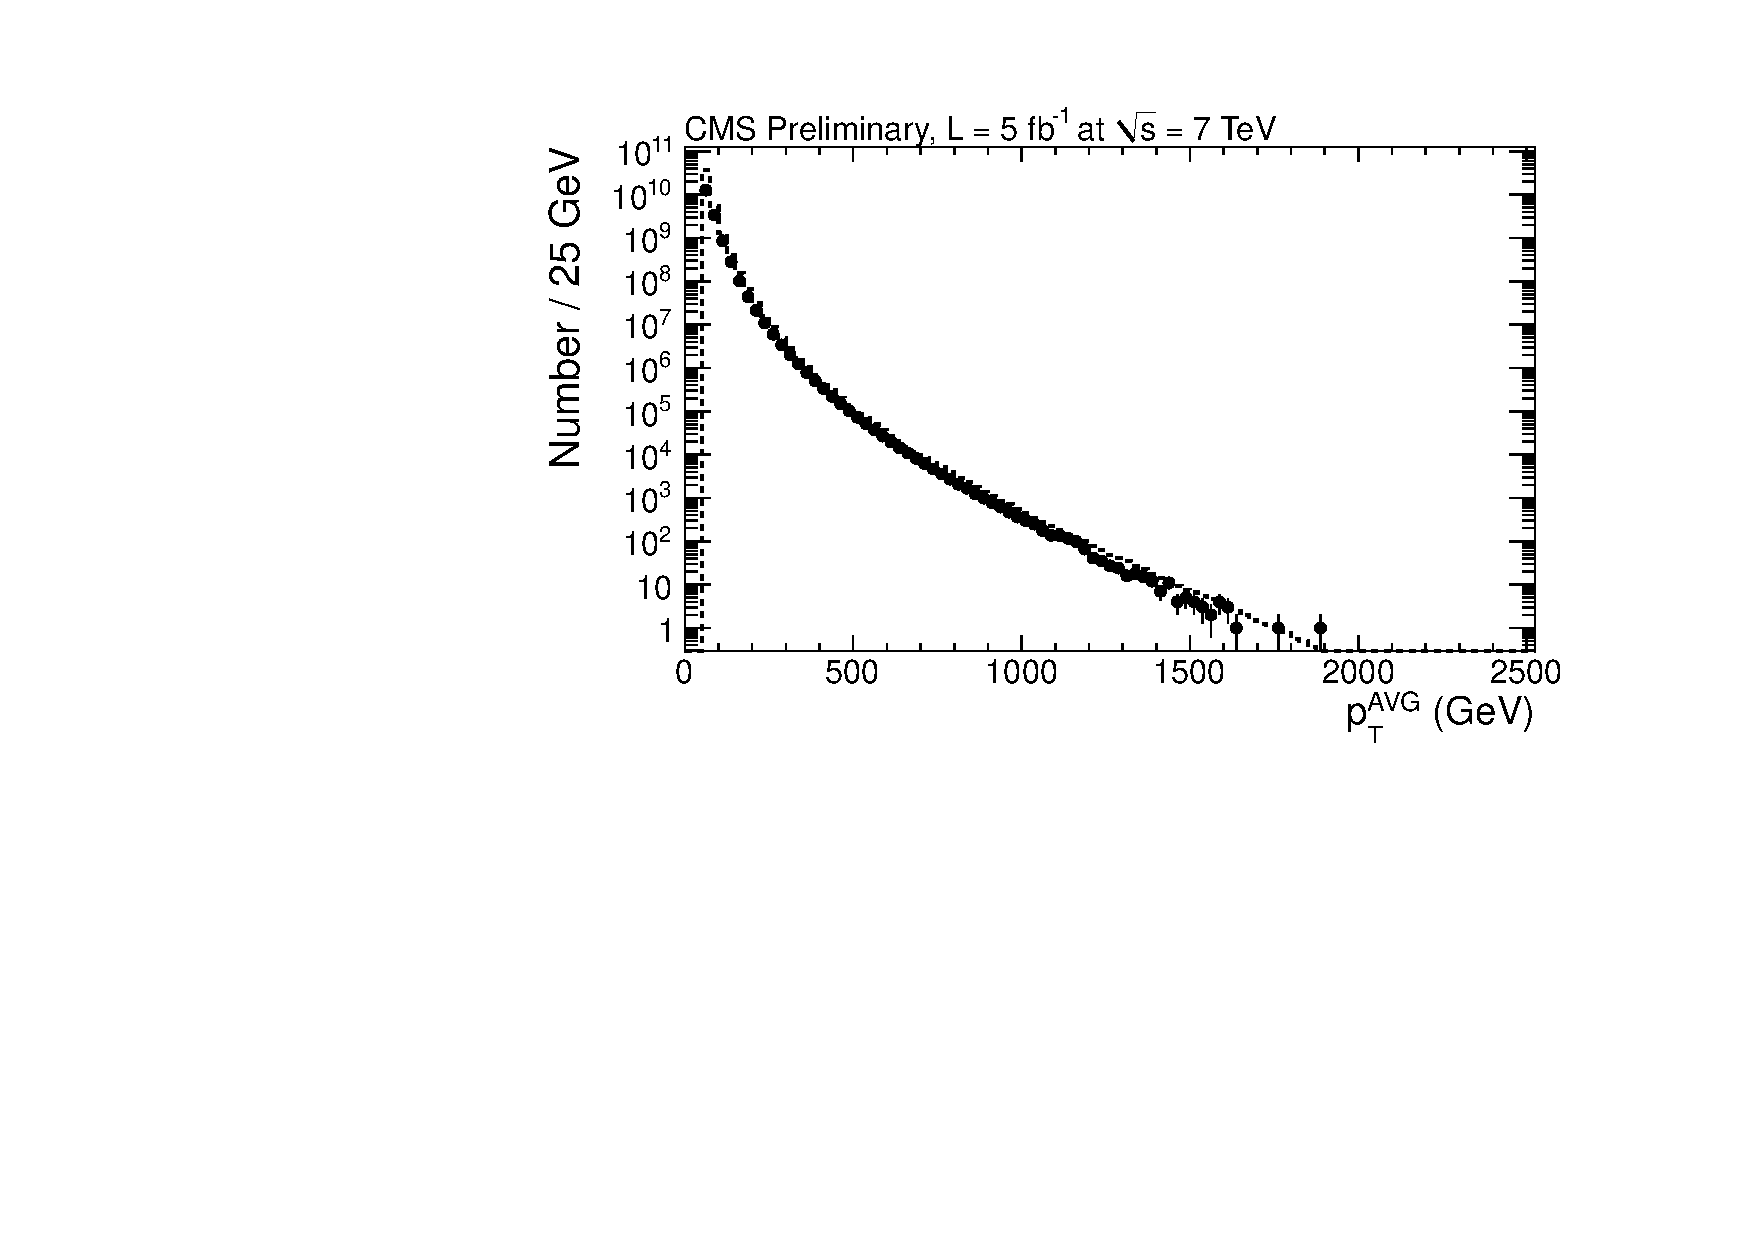
\includegraphics[width=0.95\textwidth]{figs/controlPlots_histAK7PtAvgVsNvtx}
\caption{Comparison of the $\pt^{AVG}$ distribution in data and
  \PYTHIA MC. 
\label{figs:controlPlots_histAK7PtAvgVsNvtx}}
\end{figure}



\begin{figure}[htbp]
\centering
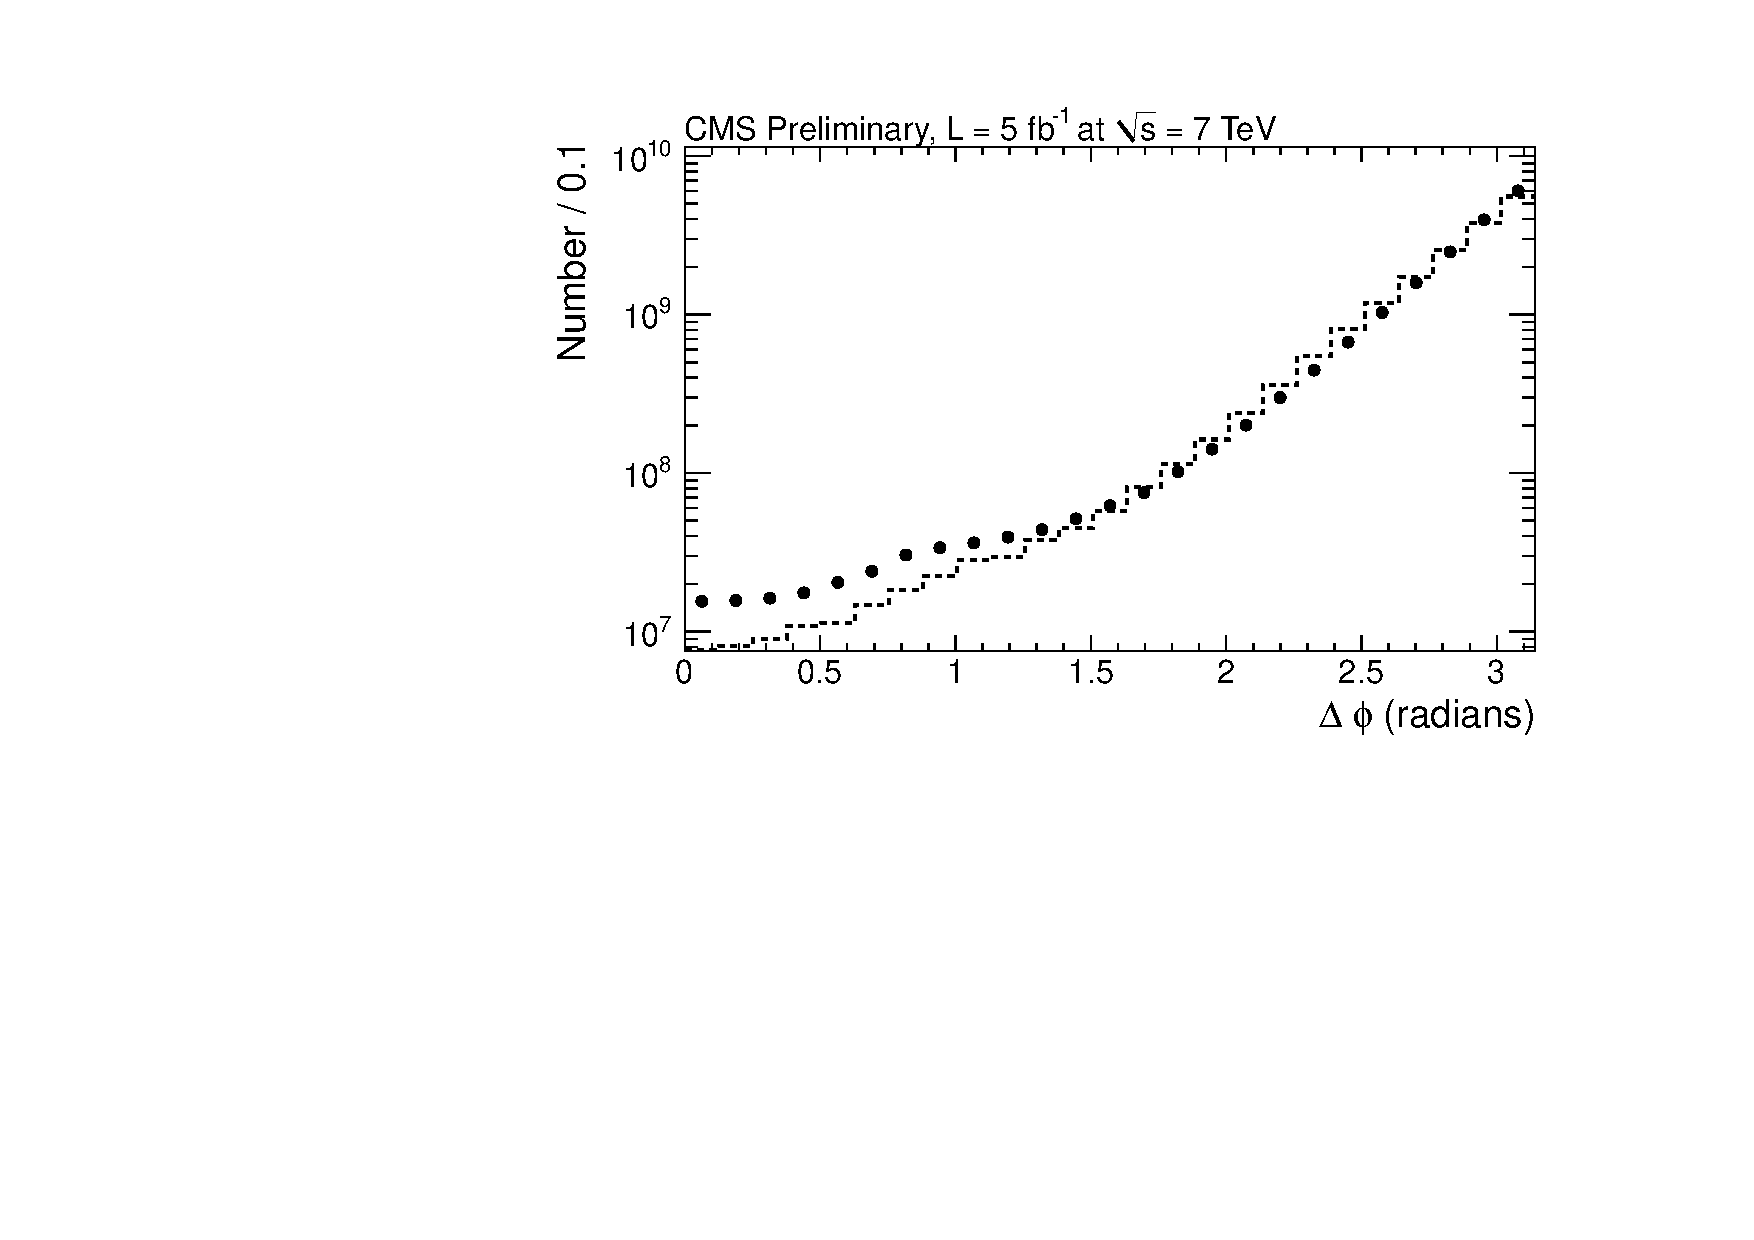
\includegraphics[width=0.95\textwidth]{figs/controlPlots_histAK7DeltaPhi}
\caption{Comparison of the $\Delta \phi$ distribution in data and
  \PYTHIA MC. 
\label{figs:controlPlots_histAK7DeltaPhi}}
\end{figure}


